\documentclass[10pt,a4paper,notitlepage,oneside,twocolumn]{abst_jsarticle}
% notitlepage : \titlepage は独立しない
% oneside : 奇数・偶数ページは同じデザイン
% twocolumn : 2段組
% \setlength{\textwidth}{\fullwidth}
% 本文領域はページ一杯で, 傍注の幅を取らない

\usepackage[dvipdfmx]{graphicx, color}
% \usepackage{amsmath}
\usepackage{amsmath,amssymb}
\usepackage{comment}
\usepackage{bm}
\usepackage{url}
\usepackage{here}
\usepackage{algorithm}
\usepackage{algpseudocode}
\usepackage{hhline} 
\usepackage[hang,small,bf]{caption}
\usepackage[subrefformat=parens]{subcaption}

% \usepackage{tabularx}
% \usepackage[dvipdfm]{graphicx}
%\numberwithin{equation}{section}

\usepackage[hmargin=2truecm, textheight= 78zw]{geometry}
\columnsep=\dimexpr \textwidth - 50zw \relax

%%\unitlength=1pt
%%\renewcommand{\baselinestretch}{0.8}

\title{
{\bf 流体シミュレーションにおけるFLIP法の粒子半径の解析}
}

\author{\begin{center}
{\large {\bf 19D8102020C 須之内 俊樹}}\\
{\large {\bf 中央大学理工学部情報工学科 形状情報処理研究室}}\\
{\large {\bf 2023年3月}}
\end{center}}

\date{}
\pagestyle{empty}

\begin{document}

\maketitle
%%%%%%%%%%%%%%%%%%%%%%%%%%%%%%


\begin{abstract}
流体シミュレーションは,流体と触れる工業製品の開発や,コンピュータグラフィックスによる流体の表現に役立っている.流体の種類や運動によって条件を設けることで,それらしい動きをシミュレーションすることができる.例えば水は非圧縮性の流体であるため,体積や密度が変化しないことが望ましい.
シミュレーションでは,様々なパラメータが登場する.シミュレーションの内容によって適切な値は異なる.本研究では,水が重力に従って運動するシミュレーションにおいて,水の体積の変化が小さくなるようなパラメータの解析を行う.
\end{abstract}

\vspace{1zw} \noindent
{\bf キーワード: }流体シミュレーション,数値流体力学,FLIP,非圧縮性条件

\section{序論} \label{sec:intro}

流体シミュレーションとは,コンピュータで流体について,流体の位置,速度,圧力などの物理量を計算し,可視化することで,流体の物理量の分布を全貌を把握する方法である.計算は流体力学の式を離散化して行う.コンピュータグラフィックスにおいては,それらしい流体の運動が高速でシミュレーションできることが重要視される.精度良く計算できることはそこまで重要視されておらず,場合によってはそれらしさのために,現実より大袈裟な表現をすることもある.

\subsection{表記法}
シミュレーションで計算する対象は,時刻ごとの,空間に分布する流体の物理量である.
流体シミュレーションの分野で一般的に使われている表記の説明をする.
\begin{quote}
	\begin{itemize}
%		\item $\bm{x}:$ 流体の位置を表すベクトル.
%		\item $t:$ 現在の時刻.
%		\item $\varDelta x,\varDelta t:$ 離散化する計算格子の格子幅,次の時刻までの時間幅.
		\item $\bm{u}(\bm{x},t):$ 位置$\bm{x}$,時刻$t$での流体の速度ベクトル.
		\item $p(\bm{x},t):$ 位置$\bm{x}$,時刻$t$での流体の圧力値.
		\item $\rho,\nu:$ それぞれ,流体の密度,流体の粘性(ここでは定数)
		\item $\bm{f}:$ 流体にかかる外力ベクトル.(簡単のため重力のみを扱い,一定の値.)
%		\item $\nabla:$ ナブラ演算子.勾配を表す.
%		\item $\frac{\rm{D}}{\rm{D}t} =\frac{\partial}{\partial t} + \bm{u(\bm{x},t)}\boldsymbol{\cdot}\nabla$ :
%		ラグランジュ微分,または物質微分.流体力学のような,連続体を扱う力学で用いられており,流れに沿って移動する物体と同じように移動する観測者から見た,物理量の時間変化率を表している.
	\end{itemize}
\end{quote}
\section{ナビエ・ストークス方程式} \label{chapter:3}
式(\ref{eq:Navie})で表されるナビエ・ストークス方程式は流体力学の支配方程式である.圧縮されない流体を扱うときは,式(\ref{eq:uncompressed})を連立させて考える.
\begin{equation}\label{eq:Navie}
\begin{split}
\frac{\partial}{\partial t}\bm{u}(\bm{x},t) = -(\bm{u}(\bm{x},t) \boldsymbol{\cdot}\nabla)\bm{u}(\bm{x},t)\\  - \frac{1}{\rho}\nabla p(\bm{x},t) + \nu\nabla^2\bm{u}(\bm{x},t) + \bm{f}
\end{split}
\end{equation}
\begin{equation}\label{eq:uncompressed}
\nabla\boldsymbol{\cdot}\bm{u}(\bm{x},t) = 0
\end{equation}

式(\ref{eq:Navie})の右辺の第一項を移流項,第二項を圧力項,第三項を粘性項,第四項を外力項とよぶ.移流項は非線形項であり,その他は線形項である.
仮の速度$\bm{u}^*$を用いて,線形項を以下の式(\ref{eq:linear}),非線形項を式(\ref{eq:nonlinear})のように分解して計算する手法がよく用いられている.
\begin{equation}\label{eq:linear}
\begin{split}
\bm{u}(\bm{x},t+1) =  \bm{u}^* - \varDelta t(\frac{1}{\rho}\nabla p(\bm{x},t)\\ + \nu\nabla^2\bm{u}(\bm{x},t) + \bm{f})
\end{split}
\end{equation} 

\begin{equation}\label{eq:nonlinear}
\bm{u}^* = \bm{u}(\bm{x},t) - \varDelta t(\bm{u}(\bm{x},t) \boldsymbol{\cdot}\nabla)\bm{u}(\bm{x},t) 
\end{equation}

空間に分布する物理量を表現し計算する手法は,大きく分けて格子法と粒子法がある.
\subsection{格子法と粒子法} \label{subsec:grid}
格子法は,流体を扱う空間を立法体の格子に区切って離散化し,格子に物理量を配置して計算する方法である.格子が規則正しく並んでいるため,微分演算を差分法などの方法で近似することができる.移流項計算の際に粘性項を取り込んで計算しているように扱うことが多いが,移流項計算の精度が悪い.

粒子法は,流体をいくつかの小さな粒子の集まりとして考え,各粒子に物理量を与えて計算をする方法である.利点として,粒子の移動によって移流項が精度よく計算できる.欠点として,粒子の影響範囲内に他の粒子がいないとき,計算がうまくできないことから,正確な物理量の分布が計算できる訳ではない.

\section{FLIP(Fluid Implicit Particles)} \label{sec:FLIP}
Harlowらの手法Particle In Cell(PIC)法\cite{PIC}は,粒子法と格子法を組み合わせた手法である.移流項の計算を粒子で行い,その他の計算を格子で行う.欠点として,通常の粒子法と比べると粒子の粘性が高くなるような効果がある.これを人工粘性と呼ぶ.BrackbillらはPICのアルゴリズムを変更し,PICの人工粘性を解消した,Fluid Implicit Particles(FLIP)法\cite{FLIP}を提案した.格子の速度を粒子の速度に受け渡す際に,粒子の速度の変化分を,粒子の速度に加算する.欠点として,数値誤差が蓄積し続けることや,粒子の勢いがほとんど減衰しないなどがある.
\section{提案手法} \label{chapter:4}
水は非圧縮性の流体なので,シミュレーションの中で密度や体積が保存されることが望ましい.本研究では,立方体の内部の領域内で,ダム崩壊シミュレーションと呼ばれる,水を柱状に配置し,重力に従って崩れるシミュレーションを行う.関数値が粒子と格子の距離が0のとき2/3,距離が大きくなるにつれて0に収束するようなカーネル関数$N(x)$を用いて,周辺の粒子からの影響を表す重みを計算する.各粒子の重みは以下のように計算し,格子の重みは格子の付近にある粒子の重みの和である.$x_p$は粒子の$x$座標,$x_i$は格子の$x$座標を表す.
\begin{equation}\label{eq:weight}
w= N(\frac{1}{h}(x_p - x_i))\boldsymbol{\cdot}N(\frac{1}{h}(y_p - y_i))\boldsymbol{\cdot}N(\frac{1}{h}(z_p - z_i))
\end{equation} 
重みに基づき閾値を定め,閾値以上の格子は液体として,液体の格子の体積を合計して流体の領域の体積を計算し,体積を保存できているかを確認する.閾値の等値面で,流体と気体の境界面を定める.
\begin{figure}[htbp]
  \begin{minipage}[b]{0.45\linewidth}
    \centering
    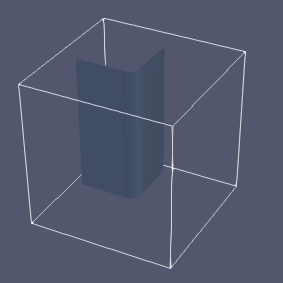
\includegraphics[width=30mm]{pirror.png}
    \caption{運動開始時の様子}
  \end{minipage}
  \begin{minipage}[b]{0.45\linewidth}
    \centering
    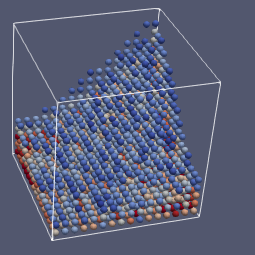
\includegraphics[width=30mm]{simulation.png}
    \caption{流体の運動の様子}
  \end{minipage}
\end{figure}

粒子の半径と,流体の非圧縮性を満たすように粒子位置の修正度を表す定数$\gamma$を用いて,粒子間の距離が近すぎるときに粒子同士を離す計算をしている.また,境界面の等値面を計算するときに用いる閾値$\theta$が,流体の体積に大きく関わる.これら三つの定数を変えてシミュレーションを行う.シミュレーション開始時の体積$V_0$と,体積の最大値$\rm{max}$と,体積の最小値$\rm{min}$を用いて,どの程度の割合で体積が変化したのかを表す$(\frac{\rm{max}}{V_0},\frac{\rm{min}}{V_0})$を計算し,その差をとることで体積の変動幅で体積が保存できているかを比較する.
\section{実験結果と考察} \label{chapter:6}

実験では,変動幅が$25\%$程度になることが確認できた.粒子半径や$\gamma$が小さいほど,体積の最小値が小さくなった.粒子位置の修正が小さく,非圧縮性を考慮していない速度の計算による移動の影響を強く受けていることが原因だと考えられる.体積が増加しているのは,シミュレーション開始から数フレーム後の,水の柱が崩れる間のみで,流体が拡散してしまっていることが確認できた.境界面での流体の拡散を防ぐ表面張力を考慮することができていないことが原因だと考えられる.
\begin{table}[h]
    \centering
    \caption{半径を格子幅の2倍にしたシミュレーションでの,体積の変動幅の初期体積に対する割合} \label{table:r2dx}
    \begin{tabular}{|l|c|c|c|}
    \hline
                			 	& $\gamma = 0.5$	 	& $\gamma =1$ 	 & $\gamma =1.5$ 		\\\hline\hline
     $\theta = 0.9$  	 & $0.4519\%$ & $0.3688\%$ & $0.2550\%$     \\
     $\theta = 0.8$      & $0.5219\%$ & $0.4052\%$ & $0.2587\%$ \\      \hline
    \end{tabular}
  \end{table}
\section{結論} \label{chapter:7}
粒子半径や$\gamma$が小さいほど,粒子の密度を修正する方向に移動する距離が小さく,体積が小さくなってしまい,非圧縮条件をよく満たしているとは言えない結果が得られた,また,表面張力の影響を考慮していなかったため,水の柱が拡散してしまい,体積が増加してしまった.FLIPは,流体シミュレーションの基本的な手法であり,抱える問題を解決している手法が多く生み出されている.今後の研究では,それらの手法についての理解を深め,シミュレーションしたい流体に適切な手法を選択できるようにするべきである.
% 参考文献
\begin{thebibliography}{99}

\bibitem{PIC}
 F.H. Harlow,(1964)The Particle-in-Cell Computing Method for Fluid Dynamics. Methods in Computational Physics,\textit{Open Journal of Modelling and Simulation},  vol.4 no.~3, pp.~319--343, July 29, 2016.

\bibitem{FLIP}
J.U.Brackbill. D.B.KotheH.M.Ruppel. Flip: A low-dissipation, particle-in-cell method for fluid flow, \textit{Computer Physics Communications}, vol.48 Issue 1, pp.25--38, January 1988.

\end{thebibliography}
\end{document}
